\section{Tecniche di compressione}
Il costo di un segnale dipende da campionamento e quantizzazione, fino ad arrivare a una quantità troppo elevata di dati per la memorizzazione ad alta qualità.

Per rappresentare l'informazione si ricorre alla compressione, cioè la trasformazione in un insieme di dati statisticamente incorrelati che garantiscano un grado di fedeltà (qualità) rispetto all'originale, e abbiano un accettabile peso computazionale per il tipo di applicazione.

Le tecniche di compressione si dividono in due grandi famiglie: lossy (con perdita accettabile a seconda dell'applicazione) e lossless (senza perdita). I dati ridondanti vengono rimossi, e il risparmio viene misurato tramite un rapporto di compressione in bit, dipendente appunto dalla ridondanza. 

I dati sono gli strumenti tramite i quali è rappresentata l'informazione, e quest'ultima può essere associata a diversi quantitativi di dati. Il principio della compressione è appunto minimizzare il numero di bit utilizzati. 
$$\text{rapporto di compressione } C = \frac{b_1 \text{ bit prima della compressione}}{b_2 \text{ bit dopo la compressione}}$$
$$\text{ridondanza relativa } R = 1 - \frac{1}{C}$$
Se $b_1 = b_2$, allora $R = 0$ e non ci sono dati ridondanti tra le due rappresentazioni. Un rapporto tipico di compressione è $10 : 1$, con corrispondente ridondanza $0.9$.

\subsection{Ridondanza}
Possono essere individuati diversi tipi di ridondanza, di cui almeno uno va ridotto:
\begin{enumerate}
	\item Della codifica;
	\item Spaziale o temporale (correlazione inter-campione);
	\item Percettiva, imponendo quantizzazioni più o meno spinte.
\end{enumerate}

I primi due consistono nella ridondanza statistica: i vicini possono essere correlati o dipendenti, quindi una parte dell'informazione è ripetuta. 

\subsubsection{Ridondanza della codifica}
La ridondanza della codifica non introduce perdita, quindi è reversibile e ha una soglia massima di compressione che può essere raggiunta. Quest'ultima dipende dal tipo di segnale.

L'idea è costruire un quantizzatore che venga usato nel miglior modo possibile, distribuendo i valori in modo equiprobabile tra i livelli. Alcuni livelli, secondo l'istogramma a livelli di grigio, hanno una maggiore probabilità di essere occupati, quindi è possibile calcolare quanto comprimere in base al numero medio normalizzato di bit necessari per ogni frequenza.

Se i valori sono sbilanciati, si ricorre alla codifica a lunghezza variabile, con numero di bit medio necessario per descrivere l'immagine:
$$L_{avg} = \sum_{k=0}^{L-1}l(r_k)p_r(r_k)$$
$l(r_k)$ è il numero di bit necessario per descrivere il $k$-esimo livello $r$, con frequenza (probabilità) $p_r$. Essendo gli standard a 256 livelli di grigio, la frequenza sarà costante e la sommatoria sarà 1, pertanto le immagini saranno codificate a $M\times N \cdot 8$ bit.

VLC (Variable-Length Coding) è una strategia di riduzione della ridondanza che impiega un numero minor di bit per rappresentare i livelli più probabili, e viceversa. Il numero medio di bit è minore rispetto alla lunghezza fissa.

\subsubsection{Ridondanza spaziale}
Quando l'istogramma è uniforme, però, la VLC non ha effetto. Tutti i valori sono equiprobabili, ma ciò li rende fortemente correlati (e pertanto ridondanti) spazialmente. Questo succede per esempio in immagini a righe, mentre lungo le colonne i valori sono incorrelati.

Si può ridurre la ridondanza spaziale individuata introducendo coppie run-length: il primo componente della coppia individua l'intensità, mentre il secondo il numero di volte con cui si ripete. L'approccio è lossless.

\subsubsection{Ridondanza percettiva}
L'immagine è percepita come se avesse un valore di grigio uniforme, ma l'istogramma è discordante da questa rappresentazione.

\begin{figure}[h]
	\centering
	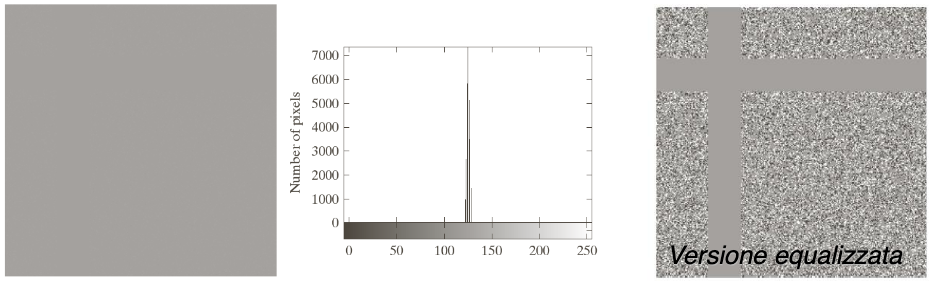
\includegraphics[scale=0.4]{Lezioni/Immagini/ridondanzapercettiva}
\end{figure}

Le informazioni ignorate dal sistema visivo umano possono essere eliminate, sostituite da un valore medio. Il processo è eseguito tramite quantizzazione, ma c'è perdita. 

\subsection{Entropia}
L'entropia è la misura della quantità di dati minima necessaria per codificare senza perdita una sorgente di informazione, modellando la sorgente come processo probabilistico con eventi statisticamente indipendenti.

Informalmente, rappresenta il valore dell'informazione attraverso incertezza e probabilità di un certo simbolo. La sorgente deve emettere valori tra di loro incorrelati, quindi non deve avere memoria. 

Nel caso delle immagini, c'è molto spesso dipendenza tra pixel contigui, ma l'entropia è la soluzione ottima a cui avvicinarsi il più possibile.

Un evento casuale $E$ con probabilità $p(E)$ ha un grado di incertezza (e una quantità di informazione) pari a:
$$I(E) = \log \frac{1}{p(E)}$$
La base del logaritmo dipende dall'unità di misura dell'informazione, in questo caso 2 (bit). Se un evento è certo, l'incertezza è nulla. 

Essendo l'entropia proporzionale all'incertezza, l'entropia di una sorgente con alfabeto $S = \{s_1, s_2, \dots,s_M\}$ è:
$$H(S) = \sum_{k=1}^{M} p_k \log_2 \frac{1}{p_k} = -\sum_{k=1}^{M}\log_2p_k$$
$p_k$ è la probabilità del $k$-esimo simbolo dell'alfabeto, e $\log_2\frac{1}{p_k}$ è la quantità di informazione contenuta nel simbolo $s_k$, cioè il numero di bit necessario per la codificaLa . situazione di equiprobabilità genera entropia massima.

L'entropia indica pertanto un limite inferiore (valore medio) per il numero di bit necessari per codificare un certo alfabeto, ipotizzando l'equiprobabilità di ogni livello e fornendo un punto di riferimento per i codici a lunghezza variabile. 

L'obiettivo di VLC è trovare il codice di lunghezza minima per descrivere il segnale. Se un codice $c_1, c_2, \dots, c_M$ ha parole con lunghezza $b_1, b_2, \dots, b_M$, il numero medio di bit richiesti è:
$$R = \sum_{k=1}^{M}b_kp_k$$
Il problema della progettazione di codice è la ricerca di parole con lunghezza media vicina all'entropia della sorgente del segnale, cioè $r$ vicino a $H$, e la stima della precisione dei valori di probabilità.

La massima entropia implica un contenuto informativo visivo basso, essendo i valori equiprobabili. Immagini diverse possono avere entropia simile, ma essa serve come valore di riferimento solo con sorgenti senza memoria, quindi il rapporto di compressione può essere molto differente in caso di fotografie o immagini con pattern.

\subsubsection{Codici di Huffman}
La codifica di Huffman funziona come VLC: ai caratteri più frequenti vengono assegnate parole di pochi bit, quindi la lunghezza è inversamente proporzionale alla probabilità.

La compressione è senza perdita, e i codici possono essere costrutiti con una struttura da albero binario, generando un codice ottimale minimizzando $L_{avg}$ in modo che sia il più vicino possibile all'entropia della sorgente.

Se il segnale viene letto sequenzialmente, non si hanno informazioni precise riguardo alla distribuzione dei simboli: essa viene stimata tramite strumenti che aggiornano a ogni valore la possibile frequenza.

\subsection{RLC}
La correlazione tra bit può portare a un elevato risparmio, ma per ottenerla si deve ricorrere a sorgenti con memoria e algoritmi come RLC  (Run-Length Coding). 

Se ci sono raggruppamenti, è possibile sfruttare la memoria codificando il simbolo con la lunghezza del corrispondente gruppo. Il segnale si presenta con tanti 0 in sequenza intervallati da 1, e viene trasmessa la coppia di valore assunto e numero di valori. 

Gran parte del contenuto informativo di un pixel è ridondante, e può essere ottenuto a partire dai pixel vicini passando a un mapping più efficiente, ma generalmente non interpretabile visivamente. 

RLC considera singolarmente le linee dell'immagine, collezionando le coppie $(g, w)$ che indicao rispettivamente il valore e la lunghezza.

Questa tecnica è impiegata per la codifica di immagini a colori, ma è poco efficiente per immagini reali a causa delle imprecisioni e del rumore. 

Il bitmap prevede una modalità di compressione senza perdita utilizzando appunto RLC, codificando le informazioni sequenziali ripetute. Il rapporto di compressione può essere minore di 1 in caso che nuovi bit vengano sprecati per creare coppie di valori diversi da quelli non contigui.

\subsection{Differential coding}
Questa tecnica viene applicata quando RLC è inefficiente, e ha come scopo la riduzione della ridondanza in simboli consecutivi di un datastream. Nel caso di audio, si utilizza la variante DPCM (Differential Pulse Code Modulation).

PCM (Pulse Code Modulation) converte forme d'onda analogiche in segnali digitali attraverso:
\begin{itemize}
	\item Campionamento;
	\item Quantizzazione;
	\item Codifica, in genere binaria.
\end{itemize}

Osservando il segnale in termine di differenza tra frequenze, una forte correlazione spaziale viene sfruttata tramite codifica a lunghezza variabile sui picchi dell'istogramma.

DCPM calcola la differenza tra frequenze adiacenti, ed essa viene codificata. Il segnale viene ricostruito sommando le differenze a partire dal valore iniziale (noto).

Nel caso delle immagini, si opera generando un'immagine differenza fra pixel contigui applicando un operatore che approssima la derivata prima (gradiente) o seconda (Laplaciana):
$$d(x, y) = I(x, y) - I(x - 1, y)$$
$$d(x, y) = 4I(x, y) - I(x, y - 1) - I(x, y + 1) - I(x + 1, y) - I(x - 1, y)$$
Per sfruttare la ridondanza tenendo conto delle differenze, è possibile anche sfruttare la differenza tra il valore attuale e quello predetto. Se la regione è uniforme in base a determinate regole, sarà immediato il calcolo del valore successivo, sfruttando l'interpolazione. 

La differenza, con valori accurati, tenderà a 0 con un istogramma stretto, e di conseguenza un'entropia minore (MPEG) in presenza di ridondanza spaziale. 

\subsection{Algoritmi lossless}
Lossless JPEG non usa la DCT e non introduce perdita utilizzando la codifica predittiva, sfruttando l'uniformità delle regioni. 

Valuta le differenze tra il valore effettivo del pixel $x$ e il suo valore predetto dai pixel adiacenti sopra e a sinistra. La sequenza di valori viene poi codificata con VLC, riportando il primo pixel identicamente. 

Gli algoritmi lossless universali non richiedono la conoscenza a priori della distribuzione di probabilità dei simboli: in genere riescono a modellare dinamicamente le caratteristiche dei dati, adeguando la codifica.

Alcuni esempi di algoritmi sono Adaptive Huffman Coding, Lempel-Ziv e Arithmetic Coding. In funzione di com'è costruita l'immagine, ciascun algoritmo sarà più o meno efficiente. 

\newpage
\subsubsection{LZW}
 \begin{wrapfigure}{R}{0.4\textwidth}
	\vspace{-15pt}
	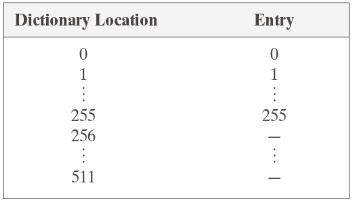
\includegraphics[width=0.4\textwidth]{Lezioni/Immagini/dizionario}
	\vspace{-20pt}
\end{wrapfigure}

LZW rimuove ridondanza di codifica e spaziale senza necessità di conoscenza a priori della probabilità di occorrenza dei simboli.

Viene inizialmente costruito un dizionario che contiene i simboli da codificare, con un ulteriore bit che permette di identificare l'occorrenza dei valori. Tutte le volte che un valore si ripete, la codifica può essere riutilizzata usando la coppia e associandola a un livello (analisi delle frequenze). 

\subsection{Codifica video}
Nei video esiste una correlazione non solo tra i pixel dello stesso fotogramma, ma anche tra fotogrammi adiacenti. In base alla ridondanza, è possibile applicare:
\begin{itemize}
	\item Compressione spaziale, intra-frame applicata a ciascuna immagine;
	\item Compressione temporale, inter-frame.
\end{itemize}

La codifica predittiva rimuove entrambe le tipologie, con un errore di predizione $e(n)$ ottenuto tramite VLC e diversi modelli di predizione.

\begin{figure}[h]
	\centering
	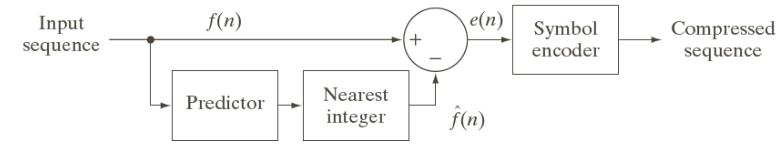
\includegraphics[scale=0.5]{Lezioni/Immagini/codificapredittiva}
\end{figure}

\subsection{Ridondanza percettiva}
In presenza di un segnale sonoro a una generica frequenza, si ha un'alterazione della soglia di udibilità per le frequenze limitrofe al segnale, che non vengono percepite: non tutta l'informazione ha la stessa importanza. 

La riduzione di ridondanza percettiva comporta quantizzazione, quindi è irreversibile e lossy dato che tiene conto solo delle componenti effettivamente udibili.

Gli schemi di compressione percettivi comprimono il segnale eliminando la parte non percepita dall'orecchio umano. Il masking può essere delle frequenze o temporale: quest'ultimo è effettuato saturando il sistema uditivo in modo da alterare le condizioni uditive (rumori forti alternati da deboli).

La ridondanza psicovisuale è un fenomeno legato alla legge di Weber: la sensibilità alle variazioni di luminosità diminuisce con la diminuzione della luminosità (immagine scura). Questo permette una maggiore quantizzazione nelle zone più scure.

L'occhio umano è più sensibile al rumore nelle regioni a bassa frequenza (uniformi) piuttosto che ad alta, e alle variazioni di luminanza piuttosto che crominanza. 

La quantizzazione IGS permette di convertire l'errore di quantizzazione alle basse frequenze in rumore ad alte frequenze, meno percepibile. L'effetto è l'eliminazione dei falsi contorni (dithering). 

I canali cromatici possono essere compressi mantenendone l'intensità, per poi ricostruire in base a questa informazione. 

\section{Valutazione della qualità di compressione}
Un sistema per la compressione di immagini è generalmente formato da unità strutturali distinte:
\begin{itemize}
	\item Codificatore o compressore:
	\begin{itemize}
		\item Di sorgente, che riduce la ridondanza del segnale operando sulle ridondanze spaziali e temporali, percettive e di codifica;
		\item Di canale, che incrementa l'immunità al rumore;
	\end{itemize}
	\item Decodificatore, che svolge le operazioni inverse:
	\begin{itemize}
		\item Di sorgente;
		\item Di canale.
	\end{itemize}
\end{itemize}

Le tecniche lossless non consentono di raggiungere rapporti di compressione superiori a $10 : 1$, effettuando solo mapping e codifica di simbolo senza quantizzazione.

La qualità della compressione si valuta una volta introdotta la quantizzazione nella fase di codifica, perché è l'unico caso in cui viene introdotta perdita di dati non ripetuti. 

La perdita di informazione permette di raggiungere rapporti fino a $100 : 1$, cercando un compromesso tra accuratezza e dimensioni. La qualità deve essere misurata quantitativamente secondo criteri oggettivi, considerando la presenza di ridondanze. 

Alcuni criteri sono:
$$\text{Segnale errore: } e(x y) = \hat{f}(x, y) - f(x, y)$$
$$\text{Errore totale: } \sum_{x=0}^{M-1} \sum_{y=0}^{N-1} e(x, y) = \sum_{x=0}^{M-1} \sum_{y=0}^{N-1} \hat{f}(x, y) - f(x, y)$$
$$\text{Root Mean Square error: } e_{rms} = \bigg[ \frac{1}{MN} \sum_{x=0}^{M-1} \sum_{y=0}^{N-1} \big[\hat{f}(x, y) - f(x, y)\big]^2\bigg]^{\frac{1}{2}}$$
$$\text{Signal to Noise Ratio: } SNR = \frac{\sum_{x=0}^{M-1} \sum_{y=0}^{N-1} \hat{f}(x, y)^2}{\sum_{x=0}^{M-1} \sum_{y=0}^{N-1} \big[\hat{f}(x, y) - f(x, y)\big]^2}$$
Il segnale errore restituisce un'immagine. RMS, il più comune, serve a normalizzare l'errore totale, dato che sommare valori di segno opposto potrebbe risultare in un numero prossimo a 0. SNR è già adottato per la quantizzazione, ma non è modellabile: è definito come il rapporto tra il segnale originale e la differenza, da minimizzare.

Le metriche non tengono in considerazione la percezione soggettiva: un algoritmo può commettere errori specifici non individuabili dalle formule, ma soltanto dall'occhio umano: sono necessari test soggettivi con valutazioni della qualità su scala predefinita e correlata con valori oggettivi. A parità di errore, una diversa tecnica di compressione potrebbe essere migliore o peggiore. 

\subsection{Codifica con trasformate}
La codifica con trasformate è un algoritmo lossy utilizzato per la compressione JPEG, che opera nel dominio trasformato. 

Trasformata diretta e inversa:
$$T(u, v) =  \sum_{x=0}^{M-1} \sum_{y=0}^{N-1} f(x, y) g(x, y, u, v)$$
$$f(x, y) = \sum_{y=0}^{M-1} \sum_{v=0}^{N-1} T(u, v) h(x, y, u, v)$$

La codifica attraverso i coefficienti della trasformata prepara alle successive fasi di compressione, in cui i coefficienti con ampiezza poco significativa sono quantizzati.

Il valore medio viene sostituito ai pixel che vengono rimossi: nel caso 2$\times$2 ci sono 4 coefficienti che vengono sostituiti da un componente, ma all'aumento del numero la correlazione tra pixel adiacenti diminuisce fino a rendere impossibile la riduzione senza perdite significative.

Diverse tipologie di coppie di trasformata e antitrasformata impiegabili:
\begin{itemize}
	\item KLT, analisi alle componenti principali, decorrela i dati ma computazionalmente inefficiente;
	\item DCT, approssima meglio il comportamento ottimo; 
	\item DFT;
	\item \dots
\end{itemize}

Viene utilizzata la trasformata lineare reversibile coseno 8$\times$8 con eliminazione di una parte dei coefficienti in base all'ampiezza, perché è il metodo che assicura un errore minore approssimando meglio il segnale a parità di numero di coefficienti. 

La dimensione $n$ della sotto-immagine è una potenza di 2 per semplicità computazionale, e all'aumentare di $n$ viene persa efficienza fino a un massimo valore di 20. Per questo motivo si preferisce 8 a 16.

64 bit permettono di rappresentare un numero di colori sufficiente, e al crescere di $n$ diminuisce la correlazione tra i pixel.

\subsection{Compressione wavelet}
I coefficienti della trasformata decorrelano il contenuto informativo dei pixel di un'immagine, permettendo una codifica più efficiente anche se con un maggior numero di operazione.

La maggior parte dell'informazione è contenuta in un numero limitato di coefficienti, e i restanti possono essere opportunamente quantizzati con scarsa influenza sulla distorsione.

Scelto il livello $J$ di analisi, la trasformata wavelet decompone l'immagine evidenziando i coefficienti legati alle caratteristiche di ogni dimensione, effettuando un'analisi statistica che evidenzia contenuto informativo legato alle basse frequenze.

Al crescere del rapporto di compressione, si ha una crescente perdita dei dettagli, in particolare texture ed edge, con conseguente smoothing, ma la qualità rispetto a DCT rimane superiore grazie all'assenza di blocchettizzazione.

Il numero di operazioni dipende dalla metodologia utilizzata (Haar, Daubechies, symlet, C-D-F) ed è  proporzionale all'efficienza. Un altro fattore importante è il numero di livelli della decomposizione wavelet, generalmente non superiore a 3.



